Asana is a project management tool used to assign tasks, impose deadlines, and track progress.
Email is \href{https://facilethings.com/blog/en/your-email-is-not-a-todo-list}{not a task management tool}.
To get started, sign up at \url{https://asana.com}.

Other potential project management tools would be the issue trackers on BitBucket and GitHub.
These support assigning tasks and accompanying discussion,
but they don't support assigning deadlines to issues, don't allow hierarchical issues (i.e., subtasks), and limit the types of supported file attachments.
You might try to use Slack as a project management tool, but I have not enjoyed it.
It is better for free-flowing conversation than keeping a to-do list.

Asana is organized into tasks, projects, and teams.
Tasks are the basic unit of work in Asana,
projects are lists of tasks, and
teams are groups of people that work together on tasks and projects.

\begin{center}
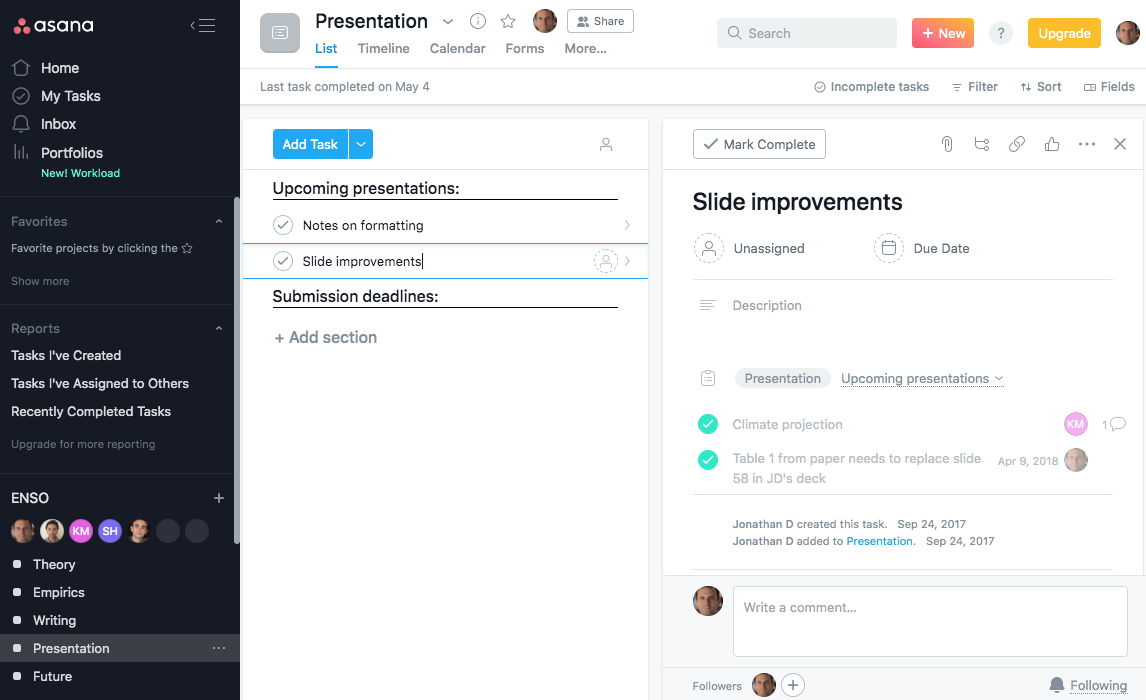
\includegraphics[width=\textwidth]{./figures/workflow/asana_screenshot1.png}
\end{center}

In this screenshot,
you see a list of projects in the left column of the ENSO workspace.
We're on the ``Presentation'' project right now, looking at a list of tasks.
One task is ``Slide improvements'', which is not assigned to anyone and lacks a due date.
It contains two subtasks:
one assigned to Kyle Meng without a due date
and
one assigned to Jonathan due April 9.
Both subtasks have been completed, so they are checked off and faded out.

To better organize projects, you can divide tasks into ``sections''.
To create a section, just create a new task within a project and end the task name with a colon.


\begin{center}
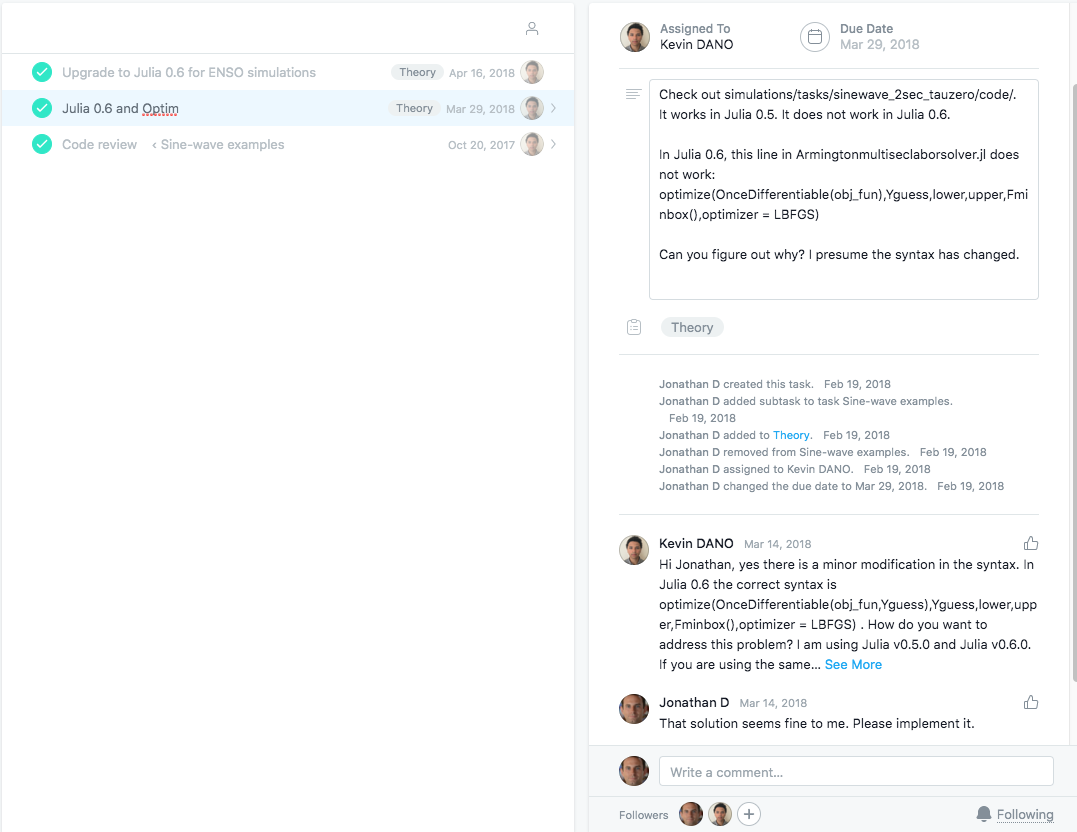
\includegraphics[width=.8\textwidth]{./figures/workflow/asana_screenshot2.png}
\end{center}

There is a comment thread associated with each task.
Asana conveniently records discussions that are categorized by task and searchable.
Kyle likely never saw the interaction in this screenshot because he was not a ``follower'' of this task.
That's good, because he was not interested in this task/conversation.
To make sure someone receives ``notifications'' related to a task in their inbox, add them as a follower.
The task assignee is automatically a follower (hence Kevin is following this task).
Commenters are automatically added as followers (hence Jonathan is also a follower).
You can grab someone's attention by using ``@'' and their name in a comment.


Jonathan loves the ``Inbox'' tab.
Following those notifications lets him track others' progress on tasks and alerts him to comments.
The ``My Tasks'' tab alerts him each day to tasks that are coming due soon.
Jonathan recommends 
(1) turning off Asana email notifications (Jonathan doesn't like email for workflow, though some of his collaborators do)
and 
(2) installing the \href{https://asana.com/apps/asana}{Asana app} on your smartphone (great way to see research progress while trapped in seminars!).



To learn more about using Asana, see these \href{https://asana.com/guide/resources/get-started/quick-start#lessons?lesson=tasks-1}{introductory lessons}.